\documentclass[8pt,aspectratio=169]{beamer}
\usetheme{Madrid}
\usepackage[utf8]{inputenc}
\usepackage[english]{babel}
\usepackage{amsmath,amssymb,amsthm}
\usepackage{graphicx}
\usepackage{tikz}
\graphicspath{{figures/}}

% Educational Warm Color Palette
\definecolor{Navy}{RGB}{30,58,138}           % #1E3A8A - Primary navy blue
\definecolor{SkyBlue}{RGB}{96,165,250}       % #60A5FA - Secondary sky blue
\definecolor{Coral}{RGB}{251,113,133}        % #FB7185 - Accent coral pink
\definecolor{Golden}{RGB}{252,211,77}        % #FCD34D - Support golden yellow
\definecolor{Cream}{RGB}{254,243,199}        % #FEF3C7 - Background cream
\definecolor{LightBlue}{RGB}{147,197,253}    % #93C5FD - Light blue variant
\definecolor{DeepCoral}{RGB}{239,68,68}      % #EF4444 - Deep coral red
\definecolor{Amber}{RGB}{251,191,36}         % #FBBF24 - Amber yellow

% Apply Educational Warm colors to beamer
\setbeamercolor{structure}{fg=Navy}
\setbeamercolor{normal text}{fg=Navy,bg=white}
\setbeamercolor{frametitle}{fg=Navy,bg=Golden!30}
\setbeamercolor{background canvas}{bg=Cream}

% Navigation and decoration
\setbeamertemplate{navigation symbols}{}
\setbeamertemplate{footline}{
  \leavevmode%
  \hbox{%
  \begin{beamercolorbox}[wd=.5\paperwidth,ht=2.5ex,dp=1ex,left]{author in head/foot}%
    \usebeamerfont{author in head/foot}\hspace{3mm}\textcolor{Navy}{Educational Warm Template}
  \end{beamercolorbox}%
  \begin{beamercolorbox}[wd=.5\paperwidth,ht=2.5ex,dp=1ex,right]{date in head/foot}%
    \usebeamerfont{date in head/foot}\textcolor{Coral}{\insertframenumber{} / \inserttotalframenumber}\hspace{3mm}
  \end{beamercolorbox}}%
  \vskip0pt%
}
\setbeamerfont{frametitle}{series=\bfseries,size=\large}

% Blocks with educational warm theme
\setbeamertemplate{blocks}[default]
\setbeamercolor{block title}{fg=white,bg=SkyBlue}
\setbeamercolor{block body}{fg=Navy,bg=LightBlue!20}
\setbeamercolor{block title alerted}{fg=white,bg=Coral}
\setbeamercolor{block body alerted}{fg=Navy,bg=Coral!15}
\setbeamercolor{block title example}{fg=white,bg=Navy}
\setbeamercolor{block body example}{fg=Navy,bg=Golden!20}

% Items with warm accent colors
\setbeamercolor{item}{fg=Coral}
\setbeamercolor{subitem}{fg=SkyBlue}
\setbeamercolor{subsubitem}{fg=Golden}
\setbeamercolor{enumerate item}{fg=Coral}
\setbeamercolor{enumerate subitem}{fg=SkyBlue}

\title{\textcolor{Navy}{Presentation Template}}
\subtitle{\textcolor{SkyBlue}{Educational Warm Layout Examples}}
\author{\textcolor{Coral}{Author Name}}
\date{}

\begin{document}

% ==================== LAYOUT 1: PLAIN TITLE ====================
\begin{frame}[plain]
\vspace{2cm}
\begin{center}
{\Huge\textcolor{Navy}{Main Title}}\\[0.5cm]
{\Large\textcolor{SkyBlue}{Subtitle or Description}}\\[2cm]
{\normalsize\textcolor{Coral}{Additional Information}}
\end{center}
\end{frame}

% ==================== LAYOUT 2: STANDARD TITLE ====================
\begin{frame}[plain]
\titlepage
\end{frame}

% ==================== LAYOUT 3: TWO COLUMNS TEXT ====================
\begin{frame}{Two Column Layout - Text}
\begin{columns}[T]
\column{0.48\textwidth}
\textcolor{Navy}{\textbf{Left Column Header}}

Main content for the left side. This is where your primary information goes.

\textcolor{Coral}{Key points:}
\begin{itemize}
\item First point
\item Second point
\item Third point with more text
\item Fourth point
\end{itemize}

Additional paragraph text can go here to provide more context or explanation.

\column{0.48\textwidth}
\textcolor{Navy}{\textbf{Right Column Header}}

Supporting content or contrasting information for the right side.

\textcolor{SkyBlue}{Related items:}
\begin{itemize}
\item Supporting point one
\item Supporting point two
\item Supporting point three
\end{itemize}

More descriptive text that complements the left column content.
\end{columns}

\vspace{\fill}
\small\textcolor{Amber}{Bottom annotation: Additional notes, references, or key takeaways}
\end{frame}

% ==================== LAYOUT 4: TWO COLUMNS WITH MATH ====================
\begin{frame}{Two Column Layout - Mathematics}
\begin{columns}[T]
\column{0.48\textwidth}
\textcolor{Navy}{\textbf{Definition}}

A mathematical concept defined:
$$\textcolor{SkyBlue}{f(x) = ax^2 + bx + c}$$

\textcolor{Coral}{Properties:}
\begin{itemize}
\item Property one: $a \neq 0$
\item Property two: Vertex at $x = -\frac{b}{2a}$
\item Property three: Discriminant $\Delta = b^2 - 4ac$
\end{itemize}

\column{0.48\textwidth}
\textcolor{Navy}{\textbf{Example}}

Specific instance:
$$\textcolor{Golden}{f(x) = 2x^2 + 3x + 1}$$

\textcolor{SkyBlue}{Calculation:}
\begin{align*}
f'(x) &= 4x + 3 \\
f'(0) &= 3 \\
f''(x) &= 4
\end{align*}

Result: Minimum at $x = -\frac{3}{4}$
\end{columns}

\vspace{\fill}
\small\textcolor{Amber}{Mathematical concepts are best understood through both theory and examples}
\end{frame}

% ==================== LAYOUT 5: EDUCATIONAL FEATURES ====================
\begin{frame}{Educational Warm Features}
\begin{columns}[T]
\column{0.48\textwidth}
\textcolor{Navy}{\textbf{Learning Elements}}

\begin{block}{Concept Introduction}
Clear presentation of new ideas with warm, inviting colors
\end{block}

\begin{alertblock}{Important Note}
Critical information highlighted with coral accents
\end{alertblock}

\begin{exampleblock}{Practice Example}
Hands-on examples with golden highlights
\end{exampleblock}

\column{0.48\textwidth}
\textcolor{SkyBlue}{\textbf{Student Engagement}}

\begin{itemize}
\item \textcolor{Coral}{Interactive} elements
\item \textcolor{SkyBlue}{Visual} learning aids
\item \textcolor{Golden}{Progressive} difficulty
\item \textcolor{Navy}{Clear} structure
\end{itemize}

\vspace{0.5em}
\textcolor{Navy}{\textbf{Learning Outcomes}}
\begin{enumerate}
\item Understand core concepts
\item Apply knowledge practically
\item Build confidence gradually
\end{enumerate}
\end{columns}

\vspace{\fill}
\small\textcolor{Amber}{Warm colors create an inviting learning environment}
\end{frame}

% ==================== LAYOUT 6: THREE-WAY SPLIT ====================
\begin{frame}{Three Column Layout}
\begin{columns}[T]
\column{0.31\textwidth}
\textcolor{Navy}{\textbf{Beginner Level}}

\textcolor{SkyBlue}{Foundation topics:}
\begin{itemize}
\item Basic concept 1
\item Basic concept 2
\item Basic concept 3
\end{itemize}

Start here for fundamentals.

\column{0.31\textwidth}
\textcolor{SkyBlue}{\textbf{Intermediate}}

\textcolor{Golden}{Building blocks:}
\begin{itemize}
\item Applied concept 1
\item Applied concept 2
\item Applied concept 3
\end{itemize}

Expand your knowledge.

\column{0.31\textwidth}
\textcolor{Coral}{\textbf{Advanced}}

\textcolor{DeepCoral}{Complex topics:}
\begin{itemize}
\item Advanced topic 1
\item Advanced topic 2
\item Advanced topic 3
\end{itemize}

Master the subject.
\end{columns}

\vspace{\fill}
\small\textcolor{Amber}{Progressive learning path from basics to mastery}
\end{frame}

% ==================== LAYOUT 7: VISUAL LEARNING ====================
\begin{frame}{Visual Learning Layout}
\textcolor{Navy}{\textbf{Concept Visualization}}

Understanding complex ideas through visual representation.

\textcolor{SkyBlue}{Key visual elements:}
\begin{itemize}
\item \textcolor{Coral}{Color coding} for different concepts
\item \textcolor{Golden}{Diagrams} to show relationships
\item \textcolor{SkyBlue}{Charts} for data representation
\end{itemize}

\vspace{0.5em}
\begin{center}
% Visual space with warm color border
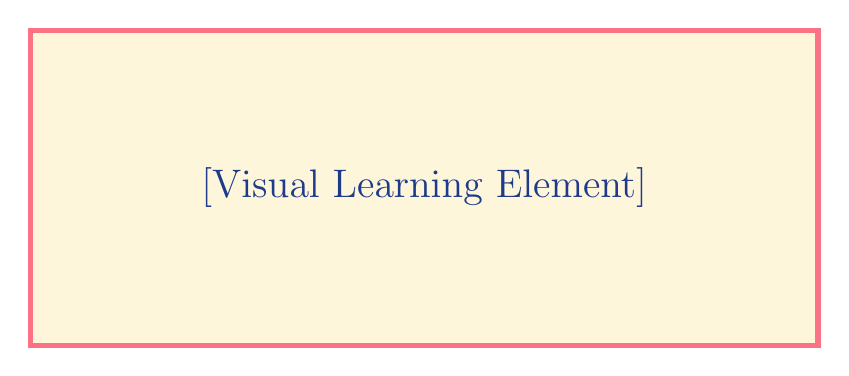
\begin{tikzpicture}
\fill[Golden!20] (0,0) rectangle (10,4);
\draw[Coral,line width=2pt] (0,0) rectangle (10,4);
\node at (5,2) {\Large\textcolor{Navy}{[Visual Learning Element]}};
\end{tikzpicture}
\end{center}

\vspace{\fill}
\small\textcolor{Amber}{Visual elements enhance comprehension and retention}
\end{frame}

% ==================== LAYOUT 8: INTERACTIVE QUIZ ====================
\begin{frame}{Interactive Quiz Format}
\begin{columns}[T]
\column{0.48\textwidth}
\textcolor{Navy}{\textbf{Question Section}}

\begin{block}{Question 1}
What is the primary purpose of this approach?
\end{block}

\textcolor{SkyBlue}{Options:}
\begin{itemize}
\item[A)] First option
\item[B)] Second option
\item[\textcolor{Coral}{C)}] Correct answer
\item[D)] Fourth option
\end{itemize}

\column{0.48\textwidth}
\textcolor{Navy}{\textbf{Explanation}}

\begin{alertblock}{Answer Key}
The correct answer is \textcolor{Coral}{\textbf{C}}
\end{alertblock}

\textcolor{Golden}{Why this answer?}
\begin{itemize}
\item Reason one
\item Reason two
\item Key insight
\end{itemize}
\end{columns}

\vspace{\fill}
\small\textcolor{Amber}{Interactive elements promote active learning}
\end{frame}

% ==================== LAYOUT 9: STEP-BY-STEP TUTORIAL ====================
\begin{frame}{Step-by-Step Tutorial}
\begin{columns}[T]
\column{0.48\textwidth}
\textcolor{Navy}{\textbf{Getting Started}}

\textcolor{SkyBlue}{\textbf{Step 1: Preparation}}
\begin{itemize}
\item Gather materials
\item Review prerequisites
\item Set up environment
\end{itemize}

\vspace{0.5em}
\textcolor{Golden}{\textbf{Step 2: Basic Practice}}
\begin{itemize}
\item Try simple example
\item Check understanding
\item Note observations
\end{itemize}

\column{0.48\textwidth}
\textcolor{Coral}{\textbf{Step 3: Application}}
\begin{itemize}
\item Apply to problem
\item Verify results
\item Document process
\end{itemize}

\vspace{0.5em}
\textcolor{DeepCoral}{\textbf{Step 4: Mastery}}
\begin{itemize}
\item Advanced techniques
\item Optimization
\item Best practices
\end{itemize}
\end{columns}

\vspace{\fill}
\small\textcolor{Amber}{Step-by-step guidance ensures systematic learning}
\end{frame}

% ==================== LAYOUT 10: KNOWLEDGE CHECK ====================
\begin{frame}{Knowledge Check}
\begin{columns}[T]
\column{0.48\textwidth}
\textcolor{Navy}{\textbf{Can You...?}}

\begin{itemize}
\item[\textcolor{Coral}{$\square$}] Define the main concept
\item[\textcolor{Coral}{$\square$}] Explain the process
\item[\textcolor{Coral}{$\square$}] Apply to new situation
\item[\textcolor{Coral}{$\square$}] Identify limitations
\item[\textcolor{Coral}{$\square$}] Compare alternatives
\end{itemize}

\vspace{0.5em}
\textcolor{SkyBlue}{\textbf{Self-Assessment}}

Rate your understanding:
\begin{itemize}
\item[\textcolor{Golden}{$\star$}] Beginner
\item[\textcolor{Golden}{$\star\star$}] Intermediate
\item[\textcolor{Golden}{$\star\star\star$}] Advanced
\end{itemize}

\column{0.48\textwidth}
\textcolor{Navy}{\textbf{Review Topics}}

\begin{block}{Strong Areas}
Topics you've mastered
\end{block}

\begin{alertblock}{Need Practice}
Areas requiring more work
\end{alertblock}

\begin{exampleblock}{Next Steps}
Recommended learning path
\end{exampleblock}
\end{columns}

\vspace{\fill}
\small\textcolor{Amber}{Regular knowledge checks reinforce learning}
\end{frame}

% ==================== LAYOUT 11: LEARNING OBJECTIVES ====================
\begin{frame}{Learning Objectives}
\begin{columns}[T]
\column{0.48\textwidth}
\textcolor{Navy}{\textbf{By the end of this lesson...}}

\textcolor{SkyBlue}{Knowledge Goals:}
\begin{itemize}
\item Understand fundamental concepts
\item Recognize key patterns
\item Identify relationships
\end{itemize}

\vspace{0.5em}
\textcolor{Golden}{Skill Goals:}
\begin{itemize}
\item Apply techniques
\item Solve problems
\item Analyze results
\end{itemize}

\column{0.48\textwidth}
\textcolor{Coral}{Competency Goals:}
\begin{itemize}
\item Evaluate approaches
\item Create solutions
\item Teach others
\end{itemize}

\vspace{0.5em}
\begin{block}{Success Criteria}
You'll be able to complete the assessment with 80\% accuracy
\end{block}
\end{columns}

\vspace{\fill}
\small\textcolor{Amber}{Clear objectives guide effective learning}
\end{frame}

% ==================== LAYOUT 12: COLLABORATIVE LEARNING ====================
\begin{frame}{Collaborative Learning}
\begin{columns}[T]
\column{0.31\textwidth}
\textcolor{Navy}{\textbf{Think}}

\textcolor{SkyBlue}{Individual reflection:}
\begin{itemize}
\item Read material
\item Form opinion
\item Note questions
\end{itemize}

Time: 2 minutes

\column{0.31\textwidth}
\textcolor{SkyBlue}{\textbf{Pair}}

\textcolor{Golden}{Partner discussion:}
\begin{itemize}
\item Share ideas
\item Compare notes
\item Resolve doubts
\end{itemize}

Time: 3 minutes

\column{0.31\textwidth}
\textcolor{Coral}{\textbf{Share}}

\textcolor{DeepCoral}{Group presentation:}
\begin{itemize}
\item Present findings
\item Get feedback
\item Build consensus
\end{itemize}

Time: 5 minutes
\end{columns}

\vspace{\fill}
\small\textcolor{Amber}{Collaborative learning enhances understanding through peer interaction}
\end{frame}

% ==================== LAYOUT 13: PRACTICAL EXERCISE ====================
\begin{frame}[fragile]{Practical Exercise}
\begin{columns}[T]
\column{0.48\textwidth}
\textcolor{Navy}{\textbf{Task Description}}

Create a function that:
\begin{itemize}
\item Takes input parameter
\item Processes data
\item Returns result
\end{itemize}

\vspace{0.5em}
\textcolor{SkyBlue}{\textbf{Starter Code}}
\begin{verbatim}
def process(data):
    # Your code here
    result = ___
    return result
\end{verbatim}

\column{0.48\textwidth}
\textcolor{Coral}{\textbf{Expected Output}}

For input: \texttt{[1, 2, 3]}\\
Output: \texttt{6}

\vspace{0.5em}
\textcolor{Golden}{\textbf{Hints}}
\begin{enumerate}
\item Consider the sum
\item Think about iteration
\item Check edge cases
\end{enumerate}

\begin{exampleblock}{Solution Available}
Check after attempting
\end{exampleblock}
\end{columns}

\vspace{\fill}
\small\textcolor{Amber}{Hands-on practice solidifies theoretical knowledge}
\end{frame}

% ==================== LAYOUT 14: CONCEPT MAP ====================
\begin{frame}{Concept Map}
\begin{center}
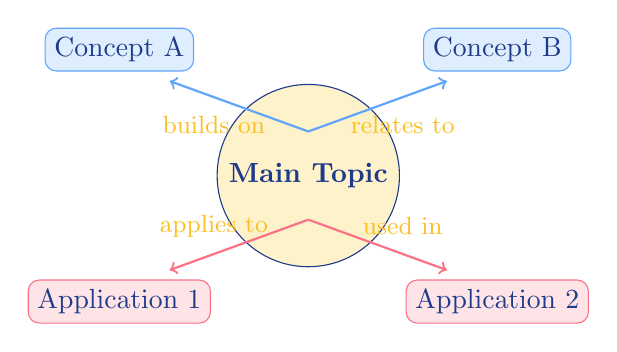
\begin{tikzpicture}[scale=0.8]
    % Central concept
    \node[draw=Navy, fill=Golden!30, circle, minimum width=2cm] at (0,0) {\textcolor{Navy}{\textbf{Main Topic}}};

    % Related concepts
    \node[draw=SkyBlue, fill=LightBlue!30, rounded corners] at (-3,2) {\textcolor{Navy}{Concept A}};
    \node[draw=SkyBlue, fill=LightBlue!30, rounded corners] at (3,2) {\textcolor{Navy}{Concept B}};
    \node[draw=Coral, fill=Coral!20, rounded corners] at (-3,-2) {\textcolor{Navy}{Application 1}};
    \node[draw=Coral, fill=Coral!20, rounded corners] at (3,-2) {\textcolor{Navy}{Application 2}};

    % Connections
    \draw[SkyBlue, thick, ->] (0,0.7) -- (-2.2,1.5);
    \draw[SkyBlue, thick, ->] (0,0.7) -- (2.2,1.5);
    \draw[Coral, thick, ->] (0,-0.7) -- (-2.2,-1.5);
    \draw[Coral, thick, ->] (0,-0.7) -- (2.2,-1.5);

    % Labels
    \node[text=Amber] at (-1.5,0.8) {\small builds on};
    \node[text=Amber] at (1.5,0.8) {\small relates to};
    \node[text=Amber] at (-1.5,-0.8) {\small applies to};
    \node[text=Amber] at (1.5,-0.8) {\small used in};
\end{tikzpicture}
\end{center}

\vspace{\fill}
\small\textcolor{Amber}{Visual concept maps reveal relationships and connections}
\end{frame}

% ==================== LAYOUT 15: SUMMARY & REVIEW ====================
\begin{frame}{Summary \& Review}
\begin{columns}[T]
\column{0.48\textwidth}
\textcolor{Navy}{\textbf{What We Learned}}
\begin{itemize}
\item \textcolor{SkyBlue}{Core concept 1}
\item \textcolor{SkyBlue}{Core concept 2}
\item \textcolor{SkyBlue}{Core concept 3}
\item \textcolor{SkyBlue}{Core concept 4}
\end{itemize}

\vspace{0.5em}
\textcolor{Golden}{\textbf{Key Takeaways}}
\begin{enumerate}
\item Main insight
\item Important principle
\item Practical application
\end{enumerate}

\column{0.48\textwidth}
\textcolor{Coral}{\textbf{Quick Quiz}}
\begin{itemize}
\item Can you explain...?
\item What happens when...?
\item How would you...?
\end{itemize}

\vspace{0.5em}
\textcolor{DeepCoral}{\textbf{Homework}}
\begin{itemize}
\item Read Chapter 5
\item Complete Exercise 3.2
\item Prepare for next class
\end{itemize}
\end{columns}

\vspace{\fill}
\small\textcolor{Amber}{Regular review reinforces learning and identifies gaps}
\end{frame}

% ==================== LAYOUT 16: RESOURCES & SUPPORT ====================
\begin{frame}{Resources \& Support}
\begin{columns}[T]
\column{0.48\textwidth}
\textcolor{Navy}{\textbf{Learning Resources}}

\textcolor{SkyBlue}{Required Reading:}
\begin{itemize}
\item Main textbook Ch. 1-3
\item Supplementary article
\item Online tutorial series
\end{itemize}

\vspace{0.5em}
\textcolor{Golden}{Additional Resources:}
\begin{itemize}
\item Video lectures
\item Practice problems
\item Discussion forum
\end{itemize}

\column{0.48\textwidth}
\textcolor{Coral}{\textbf{Getting Help}}

\textcolor{DeepCoral}{Office Hours:}
\begin{itemize}
\item Monday 2-4 PM
\item Wednesday 10-12 AM
\item By appointment
\end{itemize}

\vspace{0.5em}
\textcolor{Navy}{\textbf{Study Groups}}
\begin{itemize}
\item Tuesday evenings
\item Online sessions available
\item Peer tutoring program
\end{itemize}
\end{columns}

\vspace{\fill}
\small\textcolor{Amber}{Multiple support channels ensure student success}
\end{frame}

% ==================== LAYOUT 17: FEEDBACK & ASSESSMENT ====================
\begin{frame}{Feedback \& Assessment}
\begin{columns}[T]
\column{0.48\textwidth}
\textcolor{Navy}{\textbf{Assessment Types}}

\begin{block}{Formative}
Ongoing feedback during learning
\end{block}

\begin{alertblock}{Summative}
Final evaluation of learning
\end{alertblock}

\textcolor{SkyBlue}{\textbf{Grading Breakdown:}}
\begin{itemize}
\item Participation: 10\%
\item Assignments: 30\%
\item Midterm: 25\%
\item Final: 35\%
\end{itemize}

\column{0.48\textwidth}
\textcolor{Coral}{\textbf{Feedback Timeline}}

\begin{itemize}
\item \textcolor{Golden}{Immediate:} In-class responses
\item \textcolor{SkyBlue}{24 hours:} Quiz results
\item \textcolor{Navy}{1 week:} Assignment grades
\item \textcolor{DeepCoral}{2 weeks:} Project feedback
\end{itemize}

\vspace{0.5em}
\begin{exampleblock}{Improvement Tips}
Regular practice and timely review of feedback
\end{exampleblock}
\end{columns}

\vspace{\fill}
\small\textcolor{Amber}{Constructive feedback guides improvement}
\end{frame}

% ==================== LAYOUT 18: CLOSING MOTIVATION ====================
\begin{frame}[plain]
\vspace{2cm}
\begin{center}
{\Large\textcolor{Navy}{Great job today!}}\\[1cm]
{\huge\textcolor{Coral}{Keep Learning}}\\[0.5cm]
{\Large\textcolor{SkyBlue}{You're making excellent progress}}\\[2cm]
{\normalsize\textcolor{Golden}{See you next class!}}
\end{center}
\end{frame}

% ==================== LAYOUT 19: EDUCATIONAL WARM SPECIAL ====================
\begin{frame}{Educational Warm Color Psychology}
\begin{columns}[T]
\column{0.48\textwidth}
\textcolor{Navy}{\textbf{Why These Colors?}}

The Educational Warm palette creates:
\begin{itemize}
\item \textcolor{SkyBlue}{Trust} through calming blues
\item \textcolor{Coral}{Energy} with vibrant coral
\item \textcolor{Golden}{Optimism} from golden yellows
\item \textcolor{Cream}{Comfort} with warm backgrounds
\end{itemize}

\vspace{0.5em}
\begin{block}{Learning Impact}
Warm colors increase engagement and reduce anxiety in educational settings
\end{block}

\column{0.48\textwidth}
\textcolor{SkyBlue}{\textbf{Best Practices}}

\begin{itemize}
\item Use \textcolor{Navy}{navy} for main content
\item Apply \textcolor{Coral}{coral} for emphasis
\item Add \textcolor{Golden}{golden} highlights
\item Create \textcolor{SkyBlue}{sky blue} sections
\item Maintain \textcolor{Cream}{cream} backgrounds
\end{itemize}

\vspace{0.5em}
\begin{alertblock}{Student Feedback}
"The warm colors make learning feel more approachable and less intimidating"
\end{alertblock}
\end{columns}

\vspace{\fill}
\small\textcolor{Amber}{Educational Warm: Where learning meets comfort}
\end{frame}

% ==================== LAYOUT 20: QUICK REFERENCE ====================
\begin{frame}{Quick Reference Guide}
\begin{columns}[T]
\column{0.31\textwidth}
\textcolor{Navy}{\textbf{Formulas}}

\textcolor{SkyBlue}{Basic:}
$$y = mx + b$$

\textcolor{Golden}{Intermediate:}
$$f(x) = \int g(t)\,dt$$

\textcolor{Coral}{Advanced:}
$$\nabla^2 \phi = \rho$$

\column{0.31\textwidth}
\textcolor{SkyBlue}{\textbf{Shortcuts}}

\begin{itemize}
\item Ctrl+S: Save
\item Ctrl+Z: Undo
\item F5: Run
\item Ctrl+F: Find
\end{itemize}

\textcolor{Golden}{Pro tip:} Learn keyboard shortcuts!

\column{0.31\textwidth}
\textcolor{Coral}{\textbf{Common Errors}}

\begin{itemize}
\item Missing semicolon
\item Index out of range
\item Type mismatch
\item Null reference
\end{itemize}

\textcolor{DeepCoral}{Always check these first!}
\end{columns}

\vspace{\fill}
\small\textcolor{Amber}{Keep this reference handy during practice}
\end{frame}

\end{document}